\chapter{Evaluation and Discussion}
\label{chap:evaluation-and-discussion}

\section{Evaluation Metrics}

As NIR colorization has two main application contexts: providing human users more interpretable images and to improve object recognition results by enriching the input with more information.
To assess the effectiveness of both models, we define qualitative evaluation categories and quantitative evaluation metrics based on their ability to achieve these goals.

\subsection{Quantitative Evaluation Metrics}
Due to the unpaired setting, in the quantitative evaluation classic solutions, such as the difference between the absolute intensity values or SSIM \parencite{ssim}, cannot be applied. Fortunately, methods for comparing the general image similarity of two sets, such as FID \parencite{ttur} or
comparing classification results using an off-the-shelf network, are well known to quantitatively assess the quality of image translation.

\subsubsection*{FID}
\label{sec:fid}
To measure how close the generated images are to the real images concerning human perception, the \textit{Fréchet Inception Distance} (FID) \parencite{ttur} is a commonly used metric.
It empirically estimates how the human eye perceives images for a set of images and computes the distance between two such set representations.
First, a pre-trained InceptionV3 model evaluates each image of the image set and the activation of the last layer is considered the "human perception approximation".
Then for all activation vectors of the evaluated images in the images set, a multidimensional Gaussian is fitted over those activation vectors.
This is done for two image sets, and later the two Gaussians are compared using the Fréchet distance \parencite{ttur}.
In \autoref{fig:fid} the mechanism is visualized.
Intuitively, if the generated images are realistic, the statistics of features in a classification network should be similar to the real ones.

\begin{figure}[htp!]
    \centering
    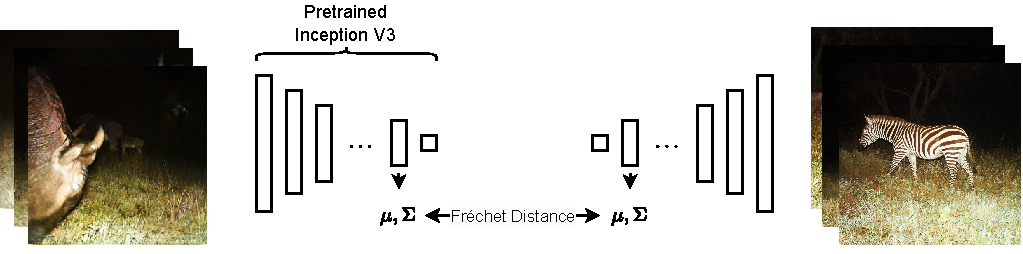
\includegraphics[width=.9\textwidth]{gfx/FID.pdf}
    \caption{
        \textbf{Fréchet Inception Distance}.
        For each image set a pretrained inception v3 model is evaluated.
        Mean $\mu$ and variance $\Sigma$ are calculated for the activations of the last layer.
        Using the Fréchet Distance a distance of between both image sets is obtained \parencite{ttur}.
    }
    \label{fig:fid}
\end{figure}

\label{sec:evaluate-fid}
\todo{Discuss usage of FID}

\subsection{Qualitative Evaluation Methods}
For qualitative evaluation, we define categories on how we determine the quality of generated images. These are again based on the two main application contexts.

The first category describes the \textit{naturality} of an image, where the generated images should resemble how humans perceive the world, without artifacts or periodic patterns that can affect visual perception.

The second category refers to the \textit{content preservation} of the input image. This should help humans as well as object detection systems to find and classify animals accurately.

\textit{Hallucinations}, as artifacts or scene elements that are not in the input image, contradict naturality and content preservation, and therefore are undesirable.

% TIMM: für jede der Kategorien wäre ein positiv und ein negativ-Beispiel hilfreich. Ansonsten wären auch Referenzen auf andere Figures möglich wo solche Fälle auftreten.

\section{Dataset Requirements}
Besides comparing both NIR colororization methods, a study on the important points for generating subsets and the suitability of each data source
(CCT and Snapshot Serengeti) as train datasets was performed.

\label{sec:time-dependent-sampling}
\label{sec:diffusion-vs-cyclegan-day}
A key factor for a good translation result is found to be the proportion between day and night images in the training dataset.
Specifically simply providing random NIR and RGB images for training of CycleGAN as well as providing random RGB images for training of the diffusion model proved to be not optimal.
As we will show, both the diffusion model and CycleGAN perform significantly worse with such a training dataset in comparison with choosing a reasonable training dataset as described in \autoref{sec:subset-generation}.

\begin{figure}[htp!]
    \centering
    \setkeys{Gin}{width=\linewidth}
    \begin{tabularx}{.7\textwidth}{Y Y Y !{\space} Y Y Y}
        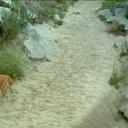
\includegraphics{gfx/unconditional-diffusion-sampling-caltech-qual/rgb_5858c0dc-23d2-11e8-a6a3-ec086b02610b.jpg} & 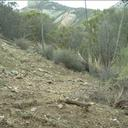
\includegraphics{gfx/unconditional-diffusion-sampling-caltech-qual/rgb_585a640e-23d2-11e8-a6a3-ec086b02610b.jpg} & 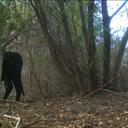
\includegraphics{gfx/unconditional-diffusion-sampling-caltech-qual/rgb_585a6486-23d2-11e8-a6a3-ec086b02610b.jpg} & 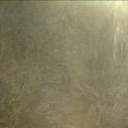
\includegraphics{gfx/unconditional-diffusion-sampling-caltech-qual/diffusion_00002.png} & 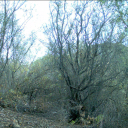
\includegraphics{gfx/unconditional-diffusion-sampling-caltech-qual/diffusion_00001.png} & 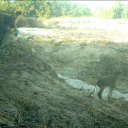
\includegraphics{gfx/unconditional-diffusion-sampling-caltech-qual/diffusion_00000.png} \\
        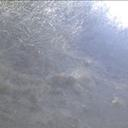
\includegraphics{gfx/unconditional-diffusion-sampling-caltech-qual/rgb_585dab96-23d2-11e8-a6a3-ec086b02610b.jpg} & 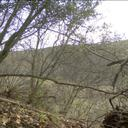
\includegraphics{gfx/unconditional-diffusion-sampling-caltech-qual/rgb_585f4d99-23d2-11e8-a6a3-ec086b02610b.jpg} & 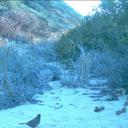
\includegraphics{gfx/unconditional-diffusion-sampling-caltech-qual/rgb_585f4fbd-23d2-11e8-a6a3-ec086b02610b.jpg} & 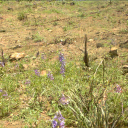
\includegraphics{gfx/unconditional-diffusion-sampling-caltech-qual/diffusion_00005.png} & 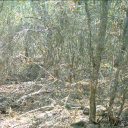
\includegraphics{gfx/unconditional-diffusion-sampling-caltech-qual/diffusion_00004.png} & 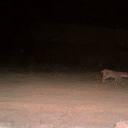
\includegraphics{gfx/unconditional-diffusion-sampling-caltech-qual/diffusion_00003.png} \\
        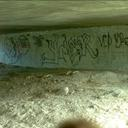
\includegraphics{gfx/unconditional-diffusion-sampling-caltech-qual/rgb_5860ef9d-23d2-11e8-a6a3-ec086b02610b.jpg} & 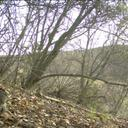
\includegraphics{gfx/unconditional-diffusion-sampling-caltech-qual/rgb_58629181-23d2-11e8-a6a3-ec086b02610b.jpg} & 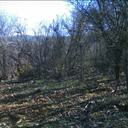
\includegraphics{gfx/unconditional-diffusion-sampling-caltech-qual/rgb_58629415-23d2-11e8-a6a3-ec086b02610b.jpg} & 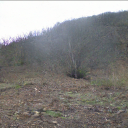
\includegraphics{gfx/unconditional-diffusion-sampling-caltech-qual/diffusion_00008.png} & 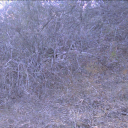
\includegraphics{gfx/unconditional-diffusion-sampling-caltech-qual/diffusion_00007.png} & 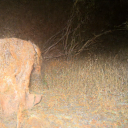
\includegraphics{gfx/unconditional-diffusion-sampling-caltech-qual/diffusion_00006.png}
    \end{tabularx}
    \caption{
        \textbf{Qualitative Evaluation of Unconditional Sampling on Caltech Dataset Subset}.
        On the left is a choice of images from the RGB domain of the test dataset, while on the right are samples produced by the unconditional diffusion model.
    }
    \label{fig:qualitative-evaluation-unconditional-sampling-caltech}
\end{figure}
% TIMM: left / right besser markieren oder abgrenzen

We train both CycleGAN and an unconditional diffusion model (acoording to \autoref{sec:methods-cycle-gan} and \autoref{sec:diffusion-prerequisites}) with a subset of the Caltech Camera Traps dataset \parencite{caltech} where \textit{randomly} from NIR and RGB images are sampled.
Secondly the same training is performed but with a dataset subset of the Serengeti dataset \parencite{serengeti} where particularly \textit{only night} images from the NIR and RGB domain are chosen.
For the diffusion model,
we achieve a FID of $100.22$ for the unconditional image generation with the \textit{random} dataset and a FID of $95.73$ with the \textit{only night} (see \autoref{sec:unconditional-diffusion-sampling-evaluation} for more information).
We consider both good results for such diverse datasets and observe that the \textit{random} dataset is more difficult to learn due to other factors.
Additionally, we provide some qualitative results for the unconditional using the model trained for the \textit{random} dataset in \autoref{fig:qualitative-evaluation-unconditional-sampling-caltech},
which also show that the trained model learned to approximate the target distribution well.
Similar results for the \textit{only-night} dataset can be found in \autoref{fig:qualitative-evaluation-unconditional-sampling} of \autoref{sec:unconditional-diffusion-sampling-evaluation}.


\begin{figure}[htp!]
    \centering
    \begin{subfigure}{\textwidth}
        \centering
        \setkeys{Gin}{width=\linewidth}
        \begin{tabularx}{\textwidth}{Y Y Y !{\space} Y Y Y}
            \multicolumn{3}{c}{Random}                                                                                     & \multicolumn{3}{c}{Only Night}                                                                                                                                                                                                                                                                                                                                                                                                                                                                                                       \\
            NIR                                                                                                            & CycleGAN                                                                                                                 & Diffusion                                                                                                            & NIR                                                                                  & CycleGAN                                                                                       & Diffusion                                                                                  \\
            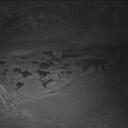
\includegraphics{gfx/conditional-diffusion-sampling-caltech-qual/nir_585a6303-23d2-11e8-a6a3-ec086b02610b.jpg} & 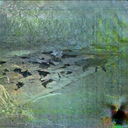
\includegraphics{gfx/conditional-diffusion-sampling-caltech-qual/cyclegan_585a6303-23d2-11e8-a6a3-ec086b02610b_fake.png} & 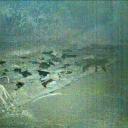
\includegraphics{gfx/conditional-diffusion-sampling-caltech-qual/diffusion_585a6303-23d2-11e8-a6a3-ec086b02610b.png} & 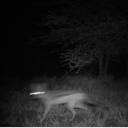
\includegraphics{gfx/conditional-diffusion-sampling-qual/nir_S2_B06_R1_PICT0128.jpg} & \includegraphics{gfx/conditional-diffusion-sampling-qual/cyclegan_S2_B06_R1_PICT0128_fake.png} & 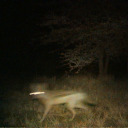
\includegraphics{gfx/conditional-diffusion-sampling-qual/diffusion_S2_B06_R1_PICT0128.png} \\
            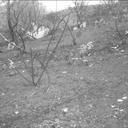
\includegraphics{gfx/conditional-diffusion-sampling-caltech-qual/nir_585c042f-23d2-11e8-a6a3-ec086b02610b.jpg} & 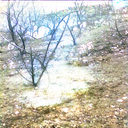
\includegraphics{gfx/conditional-diffusion-sampling-caltech-qual/cyclegan_585c042f-23d2-11e8-a6a3-ec086b02610b_fake.png} & 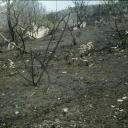
\includegraphics{gfx/conditional-diffusion-sampling-caltech-qual/diffusion_585c042f-23d2-11e8-a6a3-ec086b02610b.png} & 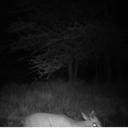
\includegraphics{gfx/conditional-diffusion-sampling-qual/nir_S2_B06_R1_PICT0387.jpg} & \includegraphics{gfx/conditional-diffusion-sampling-qual/cyclegan_S2_B06_R1_PICT0387_fake.png} & 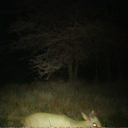
\includegraphics{gfx/conditional-diffusion-sampling-qual/diffusion_S2_B06_R1_PICT0387.png} \\
            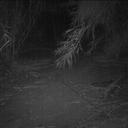
\includegraphics{gfx/conditional-diffusion-sampling-caltech-qual/nir_5860ede3-23d2-11e8-a6a3-ec086b02610b.jpg} & 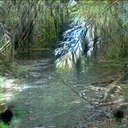
\includegraphics{gfx/conditional-diffusion-sampling-caltech-qual/cyclegan_5860ede3-23d2-11e8-a6a3-ec086b02610b_fake.png} & 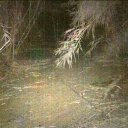
\includegraphics{gfx/conditional-diffusion-sampling-caltech-qual/diffusion_5860ede3-23d2-11e8-a6a3-ec086b02610b.png} & 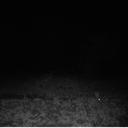
\includegraphics{gfx/conditional-diffusion-sampling-qual/nir_S2_B06_R3_PICT3848.jpg} & 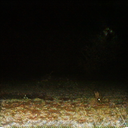
\includegraphics{gfx/conditional-diffusion-sampling-qual/cyclegan_S2_B06_R3_PICT3848_fake.png} & 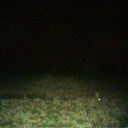
\includegraphics{gfx/conditional-diffusion-sampling-qual/diffusion_S2_B06_R3_PICT3848.png}
        \end{tabularx}
        \caption{
            \textbf{Qualitative Evaluation.}
            For each CycleGAN and the diffusion model and for each training dataset consisting of random selection of images and only night images,
            generated samples are shown.
        }
        \label{fig:hallucation-night-day-qual}
    \end{subfigure}
    \begin{subfigure}{\textwidth}
        \centering
        \begin{tabular}{c | c | c}
            Model                      & Train Dataset & FID $\downarrow$ \\
            \hline \hline
            \multirow{2}{*}{CycleGAN}  & Random        & 114.21           \\
                                       & Only Night    & \textbf{98.10}   \\
            \hline
            \multirow{2}{*}{Diffusion} & Random        & 141.77           \\
                                       & Only Night    & \textbf{96.00}   \\
        \end{tabular}
        \caption{
            \textbf{Quantitative Evaluation.}
            For each CycleGAN and the diffusion model and for each training dataset consisting of random selection of images and only night images the FID between the generated images and the respective test dataset.
        }
        \label{fig:hallucation-night-day-quan}
    \end{subfigure}
    \caption{
        Results of both CycleGAN and Diffusion when trained on a dataset consisting of \textit{only-night} images or resepectivly a \textit{random} selection of images.
        The \textit{only-night}-images dataset is obtained from the Caltech Camera Traps dataset \parencite{caltech} and the \textit{random}-images dataset is obtained from the Snapshot Serengeti dataset \parencite{serengeti}.
    }
    \label{fig:hallucincation-night-day}
\end{figure}

Starting with those four trained models we evaluate them using the respective test datasets according.
For the diffusion model we sample by replacing the high-frequencies of the intensity, as explained in \autoref{sec:correction-guided-sampling-nir-colorization} and evaluated in \autoref{sec:high-pass-filter-evaluation}.
We first conduct a qualitative evaluation of these in \autoref{fig:hallucation-night-day-qual}.
As visible, both CycleGAN and the diffusion model trained and evaluated on \textit{random} images perform much worse in \textit{content-preservation} than their equivalents trained on \textit{only-night} images.
When given dark nighttime near-infrared images, both produce features of day images, e.g., like avoiding dark sky or brightening the image.
Both model produce such features unnaturally.
Quantitative those weaknesses are also observable, we extract from \autoref{fig:hallucation-night-day-quan} that for CycleGAN the FID is 16.11 points and for the diffusion model 45.77 FID worse.

Commonly, camera traps capture near-infrared images at night and visible-light images during the day.
Therefore, sampling random NIR and RGB images results in near-infrared images mostly from the night, while the colored images are mostly from the day.

CycleGAN has its main goal of producing an image the discriminator rates as realistic.
Therefore, it hallucinates daylight features, which it learned are common for images from the dataset.
As the FID does not actually rate pictures according to their realism, but according to their distance to the target domain,
it does not necessarily rate hallucinations which do not look realistic for humans negatively.
Additionally, for CycleGAN, content-preservation is only punished by the cycle-consistency-loss, if the inverse-generator cannot recover the original image.

The diffusion model on the other hand has already proven to generate realistic images when used for unconditional sampling (\autoref{fig:qualitative-evaluation-unconditional-sampling-caltech}).
But night images are rare in its learned distribution.
Thus, it tries to generate day time images.
Our sampling procedure however, only allows sampling of color and low-frequencies of the intensity (\autoref{sec:correction-guided-sampling-nir-colorization}).
The model therefore cannot create daytime features as CycleGAN can.
As a result, we see hallucination such as images with a blue or green tone for the background,
but no details associated with these.
Notice that for day near-infrared images as the middle image in \autoref{fig:hallucation-night-day-qual}, the model does not hallucinate.
The FID again, is less effected by color changes than by differences in details and overall appearance.
Thus, the FID is much higher than CycleGAN's while we still observe hallucinations qualitatively.

In other words, both CycleGAN and the diffusion model are lead to not only translating near-infrared images to visible-light / colored images,
but also to translate from night to day. Both models fail due to different reasons in doing that.

We solve this problem, as described in \autoref{sec:subset-generation} in only providing night images for training.
As near-infrared cameras' main use case in camera traps, is to take night images we find this a reasonable decision.
When applying this to the CCT dataset \parencite{caltech} this is not actionable, because it contains too less colored night images.
Snapshot Serengeti, on the other hand, used two types of cameras during the survey:
Scoutgard's SG565 cameras which produce RGB \textbf{night} images using an \textit{incandescent} flash and
DLC Covert II cameras which use an infrared flash, and therefore produce NIR night images \parencite{serengeti}.
Thus, the Snapshot Serengeti Dataset is preferable to the CCT dataset as a training dataset for NIR to RGB night translation.

\section{Unconditional Diffusion Model}
\label{sec:unconditional-diffusion-sampling-evaluation}
First we evaluate the unconditional sampling of the diffusion model and therefore validate \parencite{diffusion-beats-gans}'s results for image synthesis in still hold for this dataset:

\begin{table}[htp!]
    \centering
    \begin{tabular}{c | c}
        Model                   & FID  $\downarrow$ \\
        \hline\hline
        CycleGAN                & 98.10             \\
        Unconditional Diffusion & 95.73
    \end{tabular}
    \caption{
        \textbf{Quantitative Evaluation of Unconditional Diffusion Sampling.} CycleGAN and the diffusion model trained on Snapshot Serengeti \parencite{serengeti} containing only night NIR and RGB images.
        Comparing the FID calculated between the test dataset and the generated images.
    }
    \label{fig:quantitative-evaluation-unconditional-sampling}
\end{table}

\begin{figure}[htp!]
    \centering
    \setkeys{Gin}{width=1\linewidth}
    \begin{tabularx}{\textwidth}{Y Y Y !{\space} Y Y Y}
        RGB                                                                                    & CycleGAN                                                                                         & Diffusion                                                                                    & RGB                                                                                    & CycleGAN                                                                                         & Diffusion                                                                                    \\
        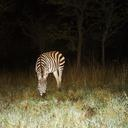
\includegraphics{gfx/unconditional-diffusion-sampling-qual/rgb_S2_B04_R3_IMAG0432.jpg} & \includegraphics{gfx/unconditional-diffusion-sampling-qual/cyclegan_S2_B06_R1_PICT0128_fake.png} & 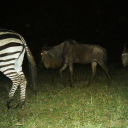
\includegraphics{gfx/unconditional-diffusion-sampling-qual/diffusion_S2_C07_R1_PICT0028.png} & 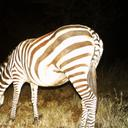
\includegraphics{gfx/unconditional-diffusion-sampling-qual/rgb_S2_B04_R3_IMAG0471.jpg} & 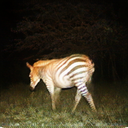
\includegraphics{gfx/unconditional-diffusion-sampling-qual/cyclegan_S2_B06_R1_PICT0279_fake.png} & 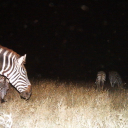
\includegraphics{gfx/unconditional-diffusion-sampling-qual/diffusion_S2_B07_R3_PICT0492.png} \\
        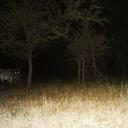
\includegraphics{gfx/unconditional-diffusion-sampling-qual/rgb_S2_B05_R1_IMAG0084.jpg} & \includegraphics{gfx/unconditional-diffusion-sampling-qual/cyclegan_S2_B06_R1_PICT0387_fake.png} & 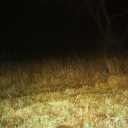
\includegraphics{gfx/unconditional-diffusion-sampling-qual/diffusion_S2_B06_R1_PICT0387.png} & 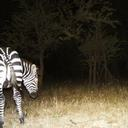
\includegraphics{gfx/unconditional-diffusion-sampling-qual/rgb_S2_B05_R1_IMAG0132.jpg} & 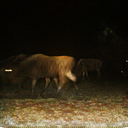
\includegraphics{gfx/unconditional-diffusion-sampling-qual/cyclegan_S2_B06_R3_PICT1364_fake.png} & 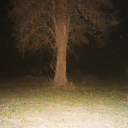
\includegraphics{gfx/unconditional-diffusion-sampling-qual/diffusion_S2_B08_R1_PICT0359.png} \\
        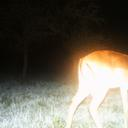
\includegraphics{gfx/unconditional-diffusion-sampling-qual/rgb_S2_B05_R2_IMAG0016.jpg} & \includegraphics{gfx/unconditional-diffusion-sampling-qual/cyclegan_S2_B06_R3_PICT3848_fake.png} & \includegraphics{gfx/unconditional-diffusion-sampling-qual/diffusion_S2_B07_R2_PICT0277.png} & \includegraphics{gfx/unconditional-diffusion-sampling-qual/rgb_S2_B05_R3_IMAG1018.jpg} & \includegraphics{gfx/unconditional-diffusion-sampling-qual/cyclegan_S2_B07_R1_PICT3274_fake.png} & \includegraphics{gfx/unconditional-diffusion-sampling-qual/diffusion_S2_B07_R1_PICT3274.png}
    \end{tabularx}
    \caption{
        \textbf{Qualitative Evaluation of Unconditional Diffusion Sampling.} Left to right: Sample image from the RGB domain of the Serengeti test dataset \parencite{serengeti},
        sample produced by CycleGAN \parencite{mehri} and an unconditional sample produced by the diffusion model \parencite{diffusion-beats-gans}.
    }
    \label{fig:qualitative-evaluation-unconditional-sampling}
\end{figure}

Qualitatively we observe in \autoref{fig:qualitative-evaluation-unconditional-sampling} that the diffusion model is capable to create realistic images.
As in the training dataset, many images without animal present are produced.
Images containing animals illustrates the model performs exceptionally well in creating realistic ones with matching lighting.
Only in few cases, trees are generated with undistinguishable branches. This is the only flaw which can be observed.

Quantitatively in \autoref{fig:quantitative-evaluation-unconditional-sampling} we see, the diffusion network only slightly outperforms CycleGAN's performance.
We expect clearer distinction to CycleGAN when a larger U-Net would be used, more training iterations and a larger dataset would be used.
Compared to \textcite{diffusion-beats-gans} we had to do trade-offs due to a lack of ultra-high performant computational resources.
Nevertheless, it can be argued that this unconditional diffusion model is capable enough to be a basis for a good colorization.

\todo{Provide hyperparameter}

\section{Loss-Guided and Correction-Guided Sampling}
As introduced in \autoref{sec:conditional-sampling} we suggest a differentiation into
\textit{loss-guided} (\autoref{sec:energy-guided-sampling}) and \textit{correction-guided} (\autoref{sec:correction-guided-sampling}) sampling.

At first sight we observe greater simplicity in defining a loss or energy rather than correcting an image.
Generally when using the correction-guided approach, the current sampled image has to be decomposed into multiple parts,
one part being the one to be modified and the second one being the remainder.
As the decomposition function must be invertible to create a functional framework, not all problems or properties are suited to be modelled like this.
Formulation as an energy is often easier to obtain and sometimes the only possibility.

In the case of near-infrared colorization both methods are implementable.
We evaluate for the context of near-infrared colorization which method should be used.
For both cases we condition using near-infrared images by assuming the intensity of the sample should be equal to the near-infrared image.
We discuss this particular conditioning method separately in \autoref{sec:nir-as-intensity-approximation-evaluation}.
In \autoref{fig:qualitative-evaluation-loss-guided-vs-correction-guided} we demonstrate the difference when formulating exactly the same property as energy-guided sampling and as correction-guided sampling.
It can be observed that the contours appear generally more noisy in the loss-guided sampling.
This observation is also quantitatively reflected, the FID of the loss-guided sampling is $23.64$ points higher than of the correction-guided approach (\autoref{fig:quantitative-evaluation-loss-guided-vs-correction-guided}).

\begin{figure}[htp!]
    \centering
    \setkeys{Gin}{width=1\linewidth}
    \begin{tabularx}{\textwidth}{Y Y Y !{\space} Y Y Y}
        \centering NIR                                                                                            & Correction-Guided                                                                                                                 & Loss-Guided                                                                                                                 & NIR                                                                                                       & Correction-Guided                                                                                                                 & Loss-Guided                                                                                                                 \\
        \includegraphics{gfx/diffusion-sampling-loss-guided-vs-correction-guided-qual/nir_S2_B06_R1_PICT0128.jpg} & \includegraphics{gfx/diffusion-sampling-loss-guided-vs-correction-guided-qual/diffusion-correction-guided_S2_B06_R1_PICT0128.png} & \includegraphics{gfx/diffusion-sampling-loss-guided-vs-correction-guided-qual/diffusion-loss-guided_S2_B06_R1_PICT0128.png} & \includegraphics{gfx/diffusion-sampling-loss-guided-vs-correction-guided-qual/nir_S2_B06_R1_PICT0279.jpg} & \includegraphics{gfx/diffusion-sampling-loss-guided-vs-correction-guided-qual/diffusion-correction-guided_S2_B06_R1_PICT0279.png} & \includegraphics{gfx/diffusion-sampling-loss-guided-vs-correction-guided-qual/diffusion-loss-guided_S2_B06_R1_PICT0279.png} \\
        \includegraphics{gfx/diffusion-sampling-loss-guided-vs-correction-guided-qual/nir_S2_B06_R1_PICT0387.jpg} & \includegraphics{gfx/diffusion-sampling-loss-guided-vs-correction-guided-qual/diffusion-correction-guided_S2_B06_R1_PICT0387.png} & \includegraphics{gfx/diffusion-sampling-loss-guided-vs-correction-guided-qual/diffusion-loss-guided_S2_B06_R1_PICT0387.png} & \includegraphics{gfx/diffusion-sampling-loss-guided-vs-correction-guided-qual/nir_S2_B06_R3_PICT1364.jpg} & \includegraphics{gfx/diffusion-sampling-loss-guided-vs-correction-guided-qual/diffusion-correction-guided_S2_B06_R3_PICT1364.png} & \includegraphics{gfx/diffusion-sampling-loss-guided-vs-correction-guided-qual/diffusion-loss-guided_S2_B06_R3_PICT1364.png} \\
        \includegraphics{gfx/diffusion-sampling-loss-guided-vs-correction-guided-qual/nir_S2_B06_R3_PICT3848.jpg} & \includegraphics{gfx/diffusion-sampling-loss-guided-vs-correction-guided-qual/diffusion-correction-guided_S2_B06_R3_PICT3848.png} & \includegraphics{gfx/diffusion-sampling-loss-guided-vs-correction-guided-qual/diffusion-loss-guided_S2_B06_R3_PICT3848.png} & \includegraphics{gfx/diffusion-sampling-loss-guided-vs-correction-guided-qual/nir_S2_B07_R1_PICT3274.jpg} & \includegraphics{gfx/diffusion-sampling-loss-guided-vs-correction-guided-qual/diffusion-correction-guided_S2_B07_R1_PICT3274.png} & \includegraphics{gfx/diffusion-sampling-loss-guided-vs-correction-guided-qual/diffusion-loss-guided_S2_B07_R1_PICT3274.png}
    \end{tabularx}
    \caption{
        \textbf{Qualitative Comparison between Correction-Guided- and Energy-Guided Sampling}.
        From left to right:
        Near-infrared image from Snapshot Serengeti dataset \parencite{serengeti},
        correction-guided sample obtained according to \autoref{sec:correction-guided-sampling-gray-scale-colorization}
        and
        energy-guided sample obtained according to \autoref{sec:energy-guided-sampling}.
        \todo{Replace loss-guided with energy guided}
    }
    \label{fig:qualitative-evaluation-loss-guided-vs-correction-guided}
\end{figure}

\begin{table}[htp!]
    \centering
    \begin{tabular}{c | c}
        Model             & FID  $\downarrow$ \\
        \hline\hline
        Correction-Guided & 105.00            \\
        Energy-Guided     & 128.64
    \end{tabular}
    \caption{
        \textbf{Quantitative Comparison between Correction-Guided- and Energy-Guided Sampling}.
        Both sampling strategies, correction-guided and energy-guided sampling is evaluated on the Snapshot Serengeti dataset \parencite{serengeti}.
        The FID (\autoref{sec:fid}) \parencite{ttur} is calculated by comparing the test dataset and the set of generated samples.
    }
    \label{fig:quantitative-evaluation-loss-guided-vs-correction-guided}
\end{table}

\todo{Provide intuition for this observation !}

\todo{Unify with observations of \autoref{sec:high-pass-filter-evaluation}}

\section{Conditioning the Near-Infrared}
\subsection{NIR as Intensity Approximation}
\label{sec:nir-as-intensity-approximation-evaluation}
\Textcite{sbgm} already suggested colorization methods using diffusion models.
Although in comparison visible light, near-infrared light has different reflection properties,
we could ignore this property and assume the NIR intensity to be a good approximation of the visual light's intensity.
Therefore, we start by implementing colorization as \autoref{sec:correction-guided-sampling-gray-scale-colorization} and evaluate
this idea empirically.

\begin{figure}[htp!]
    \centering
    \setkeys{Gin}{width=1\linewidth}
    \begin{tabularx}{\textwidth}{Y Y Y !{\space} Y Y Y}
        NIR                                                                                & CycleGAN                                                                                     & Diffusion                                                                                & NIR                                                                                & CycleGAN                                                                                     & Diffusion                                                                                \\
        \includegraphics{gfx/diffusion-sampling-intensity-qual/nir_S2_B06_R1_PICT0128.jpg} & \includegraphics{gfx/diffusion-sampling-intensity-qual/cyclegan_S2_B06_R1_PICT0128_fake.png} & \includegraphics{gfx/diffusion-sampling-intensity-qual/diffusion_S2_B06_R1_PICT0128.png} & \includegraphics{gfx/diffusion-sampling-intensity-qual/nir_S2_B06_R1_PICT0279.jpg} & \includegraphics{gfx/diffusion-sampling-intensity-qual/cyclegan_S2_B06_R1_PICT0279_fake.png} & \includegraphics{gfx/diffusion-sampling-intensity-qual/diffusion_S2_B06_R1_PICT0279.png} \\
        \includegraphics{gfx/diffusion-sampling-intensity-qual/nir_S2_B06_R1_PICT0387.jpg} & \includegraphics{gfx/diffusion-sampling-intensity-qual/cyclegan_S2_B06_R1_PICT0387_fake.png} & \includegraphics{gfx/diffusion-sampling-intensity-qual/diffusion_S2_B06_R1_PICT0387.png} & \includegraphics{gfx/diffusion-sampling-intensity-qual/nir_S2_B06_R3_PICT1364.jpg} & \includegraphics{gfx/diffusion-sampling-intensity-qual/cyclegan_S2_B06_R3_PICT1364_fake.png} & \includegraphics{gfx/diffusion-sampling-intensity-qual/diffusion_S2_B06_R3_PICT1364.png} \\
        \includegraphics{gfx/diffusion-sampling-intensity-qual/nir_S2_B06_R3_PICT3848.jpg} & \includegraphics{gfx/diffusion-sampling-intensity-qual/cyclegan_S2_B06_R3_PICT3848_fake.png} & \includegraphics{gfx/diffusion-sampling-intensity-qual/diffusion_S2_B06_R3_PICT3848.png} & \includegraphics{gfx/diffusion-sampling-intensity-qual/nir_S2_B07_R1_PICT3274.jpg} & \includegraphics{gfx/diffusion-sampling-intensity-qual/cyclegan_S2_B07_R1_PICT3274_fake.png} & \includegraphics{gfx/diffusion-sampling-intensity-qual/diffusion_S2_B07_R1_PICT3274.png}
    \end{tabularx}
    \caption{
        \textbf{Qualitative Evaluation of Intensity Replacement Sampling.}
        From left to right:
        Near-infrared image from Snapshot Serengeti dataset \parencite{serengeti},
        image generated by CycleGAN (\autoref{sec:methods-cycle-gan})\parencite{mehri}
        and
        sample obtained using intensity replacement as conditioning strategy according to \autoref{sec:correction-guided-sampling-gray-scale-colorization}.
    }
    \label{fig:qualitative-evaluation-intensity}
\end{figure}

In \autoref{fig:qualitative-evaluation-intensity} we show evaluation results of this approach.
Qualitatively we can observe those generated images are faithful to the input image (\autoref{fig:qualitative-evaluation-intensity}).
It is to be mentioned that faithfulness to the input image is not a quality learned by the network, but a design choice of the sampling procedure.
Most noteworthy is that the colors estimated by the diffusion model appear realistic.
Qualitative weaknesses in the colorization can be observed when analyzing the zebra image:
While CycleGAN colorizes the main zebra body as black and white, the diffusion network produces an orange-black zebra.
This can be traced back to a conceptional weakness.
The diffusion network is forced to reuse the intensity of the NIR image.
The zebra in the NIR image is gray-black and therefore the network is not capable in generating high intensity pixels.
CycleGAN on the other-hand is not restricted by design to change the intensity.
It is merely trained to produce invertible images.

\begin{table}[htp!]
    \centering
    \begin{tabular}{c | c}
        Model                                           & FID  $\downarrow$ \\
        \hline\hline
        CycleGAN                                        & 98.10             \\
        Unconditional Diffusion                         & 96.03             \\
        \textbf{Conditional Diffusion} \parencite{sbgm} & \textbf{105.00}
    \end{tabular}
    \caption{
        \textbf{Quantitative Evaluation of Intensity Replacement Sampling.}
        Samples of CycleGAN, the unconditional diffusion model and conditional diffusion model using intensity replacement sampling are generated.
        The FID (\autoref{sec:fid}) \parencite{ttur} is calculated by comparing the test dataset and the set of generated samples.
    }
    \label{fig:qualitative-evaluation-full-high-pass}
\end{table}


Similar to the minor qualitative weakness, we also observe the FID of this naive approach to be $6.9$ FID points worse than CycleGAN.
Additionally, we see a gap between the sampling the unconditional diffusion model produces our method according to \Citeauthor*{sbgm} of $8.97$ FID points \parencite{sbgm}.
This indicates that this method is too restrictive to allow competitive image generation.


\todo{Explanation why approximation even works, night, few vegetation, ...}

To improve the intuition of the difference between the intensities, we consider CycleGAN's intensities a good approximation of the real visible intensity.
We compare this with the near-infrared intensity in \autoref{fig:heatmap-cycle-gan-intensity}.

\begin{figure}[htp!]
    \centering
    \includegraphics[width=\textwidth]{gfx/heatmap-nir-cycle-gan-intensity-diff.pdf}
    \caption{
        \todo{Better integration (using pdf or so); Best: Direct latex code}
        Absolute difference between CycleGAN's intensity and the NIR image.
        Left to Right: Intensity calculated by images generated by CycleGAN, Near-Infared image \parencite{serengeti} and difference between both.
    }
    \label{fig:heatmap-cycle-gan-intensity}
\end{figure}

We first observe the pattern, that CycleGAN does especially enlighten the foreground and with that the lower regions of the image.
The same holds for animals in the foreground such as the fox or zebra.
Indeed, while comparing the intensity of near-infrared and the incandescent image in the Serengeti dataset \parencite{serengeti}
this pattern is observable again:
Generally the light in incandescent images appears to be stronger and therefore foreground objects are more illuminated.

Naturally when fixing the intensity of the NIR image for the diffusion sampling, such distinct features of the incandescent images is not achievable,
and therefore a higher FID is not unexpected.

As it is now clear that this physical inaccuracy we accepted, might influence the performance of our sampling, it is not yet clear to what extent.
To investigate this, in \autoref{fig:qualitative-evaluation-cyclegan-conditional-sampling} choose to use the same sampling method as before, but instead use the intensities produced by CycleGAN as input to the diffusion sampling.

\begin{figure}[htp!]
    \centering
    \setkeys{Gin}{width=1\linewidth}
    \begin{tabularx}{\textwidth}{Y Y Y !{\space} Y Y Y}
        NIR                                                                              & CycleGAN                                                                                   & Diffusion with CycleGAN Input                                                                    & NIR                                                                              & CycleGAN                                                                                   & Diffusion with CycleGAN Input                                                                    \\
        \includegraphics{gfx/conditional-with-cycle-gan-qual/nir_S2_B06_R1_PICT0128.jpg} & \includegraphics{gfx/conditional-with-cycle-gan-qual/cyclegan_S2_B06_R1_PICT0128_fake.png} & \includegraphics{gfx/conditional-with-cycle-gan-qual/diff_cycle_gan_S2_B06_R1_PICT0128_fake.png} & \includegraphics{gfx/conditional-with-cycle-gan-qual/nir_S2_B06_R1_PICT0279.jpg} & \includegraphics{gfx/conditional-with-cycle-gan-qual/cyclegan_S2_B06_R1_PICT0279_fake.png} & \includegraphics{gfx/conditional-with-cycle-gan-qual/diff_cycle_gan_S2_B06_R1_PICT0279_fake.png} \\
        \includegraphics{gfx/conditional-with-cycle-gan-qual/nir_S2_B06_R1_PICT0387.jpg} & \includegraphics{gfx/conditional-with-cycle-gan-qual/cyclegan_S2_B06_R1_PICT0387_fake.png} & \includegraphics{gfx/conditional-with-cycle-gan-qual/diff_cycle_gan_S2_B06_R1_PICT0387_fake.png} & \includegraphics{gfx/conditional-with-cycle-gan-qual/nir_S2_B06_R3_PICT1364.jpg} & \includegraphics{gfx/conditional-with-cycle-gan-qual/cyclegan_S2_B06_R3_PICT1364_fake.png} & \includegraphics{gfx/conditional-with-cycle-gan-qual/diff_cycle_gan_S2_B06_R3_PICT1364_fake.png} \\
        \includegraphics{gfx/conditional-with-cycle-gan-qual/nir_S2_B06_R3_PICT3848.jpg} & \includegraphics{gfx/conditional-with-cycle-gan-qual/cyclegan_S2_B06_R3_PICT3848_fake.png} & \includegraphics{gfx/conditional-with-cycle-gan-qual/diff_cycle_gan_S2_B06_R3_PICT3848_fake.png} & \includegraphics{gfx/conditional-with-cycle-gan-qual/nir_S2_B07_R1_PICT3274.jpg} & \includegraphics{gfx/conditional-with-cycle-gan-qual/cyclegan_S2_B07_R1_PICT3274_fake.png} & \includegraphics{gfx/conditional-with-cycle-gan-qual/diff_cycle_gan_S2_B07_R1_PICT3274_fake.png}
    \end{tabularx}
    \caption{
        \textbf{Qualitative Evaluation of Intensity Replacement Sampling For Given Intensity.}
        From left to right:
        Near-infrared image from Snapshot Serengeti dataset \parencite{serengeti},
        image generated by CycleGAN (\autoref{sec:methods-cycle-gan})\parencite{mehri}
        and
        sample obtained using intensity replacement as conditioning strategy, but with intensity from CycleGAN (\autoref{sec:correction-guided-sampling-gray-scale-colorization}).
    }
    \label{fig:qualitative-evaluation-cyclegan-conditional-sampling}
\end{figure}

\begin{table}[htp!]
    \centering
    \begin{tabular}{c | c}
        Model                                    & FID  $\downarrow$ \\
        \hline\hline
        CycleGAN                                 & 98.10             \\
        Diffusion with CycleGAN Intensity Inputs & \textbf{97.21}    \\
        Diffusion with NIR Inputs                & 104.04
    \end{tabular}
    \caption{
        \textbf{Quantitative Evaluation of Intensity Replacement Sampling.}
        Samples are obtained from CycleGAN, the diffusion model given CycleGAN's intensities and the diffusion model with NIR inputs.
        The FID (\autoref{sec:fid}) \parencite{ttur} is calculated by comparing the test dataset and the set of generated samples.
    }
    \label{fig:quantitative-evaluation-cyclegan-conditional-sampling}
\end{table}


In \autoref{fig:qualitative-evaluation-cyclegan-conditional-sampling} we see that not only is the diffusion model more than capable in colorizing these pictures,
it also exceeds CycleGAN's color choices. While the zebra of CycleGAN has an orange outline at the head where it should not, the diffusion model does not make this mistake
which results in overall more realistic images.

This subtle difference between the CycleGAN and the diffusion model samples with CycleGAN intensity inputs is also visible while comparing the images quantitatively in \autoref{fig:quantitative-evaluation-cyclegan-conditional-sampling}.
The diffusion model performs better than CycleGAN when the intensities are appropriate.
Diffusion models theoretically perform best in the unconditional sampling in comparison when they being guided by unseen data.
In the unconditional setting it only performs $1.2$ FID points better (\autoref{fig:quantitative-evaluation-unconditional-sampling}).
Therefore, we have shown that the assumption that the near-infrared intensities approximate the visual intensities well,
is the main factor explaining the difference between the quantitative results.

\subsection{High-Pass Filtering of NIR}
\label{sec:high-pass-filter-evaluation}

To improve this weakness, we can get inspired by simple NIR-RGB enhancement methods based on filters \parencite{rgb-nir-image-enhancement}.
A better approximation is to use only the high-frequencies of the near-infrared image while the low frequencies can still be sampled by the diffusion model (\autoref{sec:correction-guided-sampling-nir-colorization}).
This intuitively also gives the diffusion model freedom to sample different illumination than given by the near-infrared image.

In \autoref{fig:qualitative-evaluation-full-high-pass} we evaluate the results of this concept.

\begin{figure}[htp!]
    \centering
    \setkeys{Gin}{width=1\linewidth}
    \begin{tabularx}{\textwidth}{Y Y Y !{\space} Y Y Y}
        NIR                                                                                               & Full-Pass                                                                                               & High-Pass                                                                                               & NIR                                                                                               & Full-Pass                                                                                               & High-Pass                                                                                               \\
        \includegraphics{gfx/diffusion-sampling-full-vs-high-pass-filter-qual/nir_S2_B06_R1_PICT0128.jpg} & \includegraphics{gfx/diffusion-sampling-full-vs-high-pass-filter-qual/full-pass_S2_B06_R1_PICT0128.png} & \includegraphics{gfx/diffusion-sampling-full-vs-high-pass-filter-qual/high-pass_S2_B06_R1_PICT0128.png} & \includegraphics{gfx/diffusion-sampling-full-vs-high-pass-filter-qual/nir_S2_B06_R1_PICT0279.jpg} & \includegraphics{gfx/diffusion-sampling-full-vs-high-pass-filter-qual/full-pass_S2_B06_R1_PICT0279.png} & \includegraphics{gfx/diffusion-sampling-full-vs-high-pass-filter-qual/high-pass_S2_B06_R1_PICT0279.png} \\
        \includegraphics{gfx/diffusion-sampling-full-vs-high-pass-filter-qual/nir_S2_B06_R1_PICT0387.jpg} & \includegraphics{gfx/diffusion-sampling-full-vs-high-pass-filter-qual/full-pass_S2_B06_R1_PICT0387.png} & \includegraphics{gfx/diffusion-sampling-full-vs-high-pass-filter-qual/high-pass_S2_B06_R1_PICT0387.png} & \includegraphics{gfx/diffusion-sampling-full-vs-high-pass-filter-qual/nir_S2_B06_R3_PICT1364.jpg} & \includegraphics{gfx/diffusion-sampling-full-vs-high-pass-filter-qual/full-pass_S2_B06_R3_PICT1364.png} & \includegraphics{gfx/diffusion-sampling-full-vs-high-pass-filter-qual/high-pass_S2_B06_R3_PICT1364.png} \\
        \includegraphics{gfx/diffusion-sampling-full-vs-high-pass-filter-qual/nir_S2_B06_R3_PICT3848.jpg} & \includegraphics{gfx/diffusion-sampling-full-vs-high-pass-filter-qual/full-pass_S2_B06_R3_PICT3848.png} & \includegraphics{gfx/diffusion-sampling-full-vs-high-pass-filter-qual/high-pass_S2_B06_R3_PICT3848.png} & \includegraphics{gfx/diffusion-sampling-full-vs-high-pass-filter-qual/nir_S2_B07_R1_PICT3274.jpg} & \includegraphics{gfx/diffusion-sampling-full-vs-high-pass-filter-qual/full-pass_S2_B07_R1_PICT3274.png} & \includegraphics{gfx/diffusion-sampling-full-vs-high-pass-filter-qual/high-pass_S2_B07_R1_PICT3274.png}
    \end{tabularx}
    \caption{
        \textbf{Qualitative Evaluation of High-Frequency Intensity Replacement.}
        From left to right:
        Near-infrared image from Snapshot Serengeti dataset \parencite{serengeti},
        sample obtained using intensity replacement as conditioning strategy (\autoref{sec:correction-guided-sampling-gray-scale-colorization})
        and
        image generated using replacement of high-frequency intensities (\autoref{sec:correction-guided-sampling-nir-colorization}).
    }
    \label{fig:qualitative-evaluation-full-high-pass}
\end{figure}

\begin{table}[htp!]
    \centering
    \begin{tabular}{c | c}
        Strategy                             & FID  $\downarrow$ \\
        \hline\hline
        Intensity Replacement                & 105.00            \\
        High-Frequency Intensity Replacement & 95.49             \\
        Unconditional                        & 96.02
    \end{tabular}
    \caption{
        \textbf{Quantitative Evaluation of High-Frequency Intensity Replacement Sampling.}
        Images are generated using intensity replacement sampling, high-frequency intensity replacement and unconditionally.
        The FID (\autoref{sec:fid}) \parencite{ttur} is calculated by comparing the test dataset and the set of generated samples.
    }
    \label{fig:quantitative-evaluation-full-high-pass}
\end{table}


As expected the diffusion now using the high-pass filter can manipulate the illumination of the scene.
For example, we observe for left top image now, that not only the fox itself but also the environment has an orange-lighting as typically found in the training dataset.
This reduction in restriction also positively influences the quantitative measurements:
This method achieves a FID of $95.49$ which is even $0.53$ FID points better than the unconditional sampling (\autoref{fig:quantitative-evaluation-full-high-pass}).

\todo{Resolve conflict to statement: "unconditional sampling is always the best" }

\todo{Discuss the qualitative negative points $\rightarrow$ hallucinations}

\subsection{Influence of Hyperparameter Sigma}
\label{sec:influence-of-sigma-evaluation}

While introducing the hyperparameter $\sigma$ in \autoref{sec:correction-guided-sampling-nir-colorization}, we further want to discuss its influence on the samples.
As $\sigma$ controls the strength of the Gaussian-filter for the low-frequency extraction, increasing it, reduces information in the extracted low-frequencies.
Vice versa raising $\sigma$, leads to more information in the extracted high-frequencies.
We visualize this effect in \autoref{fig:low-and-high-freq-effects-of-sigma}.


\begin{figure}[htp!]
    \centering
    \setkeys{Gin}{width=1\linewidth}
    \begin{tabularx}{.6\textwidth}{>{\centering\arraybackslash}m{.08\linewidth} Y Y Y}
                                                                    & $\sigma=1$                                                           & $\sigma=5$                                                           & $\sigma=10$                                                           \\
        \begin{sideways}\makecell{Low-\\Frequencies}\end{sideways}  & \includegraphics{gfx/low-high-freq-effects-of-sigma/low_freq_1.png}  & \includegraphics{gfx/low-high-freq-effects-of-sigma/low_freq_5.png}  & \includegraphics{gfx/low-high-freq-effects-of-sigma/low_freq_10.png}  \\
        \begin{sideways}\makecell{High-\\Frequencies}\end{sideways} & \includegraphics{gfx/low-high-freq-effects-of-sigma/high_freq_1.png} & \includegraphics{gfx/low-high-freq-effects-of-sigma/high_freq_5.png} & \includegraphics{gfx/low-high-freq-effects-of-sigma/high_freq_10.png} \\
    \end{tabularx}

    \caption{
        \textbf{Influence of $\mathbf{\sigma}$ to low- and high-frequencies}.
        Top row: Low Frequencies parts of image, bottom row: high-frequency part of image.
        From left to right: Decomposition into low- and high frequencies according to \autoref{sec:correction-guided-sampling-nir-colorization} for $\sigma=1$, $\sigma=5$ and $\sigma=10$.
    }
    \label{fig:low-and-high-freq-effects-of-sigma}
\end{figure}

Recall, high-frequency intensities of the near-infrared are combined with the generated low-frequency intensities.
Therefore, a higher $\sigma$ also corresponds to more guidance by the near-infrared image.
On the other hand lower $\sigma$ corresponds to more freedom in generation for the model.

In \autoref{fig:quantitative-evaluation-influence-of-sigma-to-fid} we visualize the effects of $\sigma$ on the FID.
We evaluate with the same seed, with the intention to have as few influence of randomness as possible.

\begin{figure}[htp!]
    \begin{center}
        %% Creator: Matplotlib, PGF backend
%%
%% To include the figure in your LaTeX document, write
%%   \input{<filename>.pgf}
%%
%% Make sure the required packages are loaded in your preamble
%%   \usepackage{pgf}
%%
%% Also ensure that all the required font packages are loaded; for instance,
%% the lmodern package is sometimes necessary when using math font.
%%   \usepackage{lmodern}
%%
%% Figures using additional raster images can only be included by \input if
%% they are in the same directory as the main LaTeX file. For loading figures
%% from other directories you can use the `import` package
%%   \usepackage{import}
%%
%% and then include the figures with
%%   \import{<path to file>}{<filename>.pgf}
%%
%% Matplotlib used the following preamble
%%   \usepackage{fontspec}
%%
\begingroup%
\makeatletter%
\begin{pgfpicture}%
\pgfpathrectangle{\pgfpointorigin}{\pgfqpoint{6.400000in}{4.800000in}}%
\pgfusepath{use as bounding box, clip}%
\begin{pgfscope}%
\pgfsetbuttcap%
\pgfsetmiterjoin%
\definecolor{currentfill}{rgb}{1.000000,1.000000,1.000000}%
\pgfsetfillcolor{currentfill}%
\pgfsetlinewidth{0.000000pt}%
\definecolor{currentstroke}{rgb}{1.000000,1.000000,1.000000}%
\pgfsetstrokecolor{currentstroke}%
\pgfsetdash{}{0pt}%
\pgfpathmoveto{\pgfqpoint{0.000000in}{0.000000in}}%
\pgfpathlineto{\pgfqpoint{6.400000in}{0.000000in}}%
\pgfpathlineto{\pgfqpoint{6.400000in}{4.800000in}}%
\pgfpathlineto{\pgfqpoint{0.000000in}{4.800000in}}%
\pgfpathlineto{\pgfqpoint{0.000000in}{0.000000in}}%
\pgfpathclose%
\pgfusepath{fill}%
\end{pgfscope}%
\begin{pgfscope}%
\pgfsetbuttcap%
\pgfsetmiterjoin%
\definecolor{currentfill}{rgb}{1.000000,1.000000,1.000000}%
\pgfsetfillcolor{currentfill}%
\pgfsetlinewidth{0.000000pt}%
\definecolor{currentstroke}{rgb}{0.000000,0.000000,0.000000}%
\pgfsetstrokecolor{currentstroke}%
\pgfsetstrokeopacity{0.000000}%
\pgfsetdash{}{0pt}%
\pgfpathmoveto{\pgfqpoint{0.800000in}{0.528000in}}%
\pgfpathlineto{\pgfqpoint{5.760000in}{0.528000in}}%
\pgfpathlineto{\pgfqpoint{5.760000in}{4.224000in}}%
\pgfpathlineto{\pgfqpoint{0.800000in}{4.224000in}}%
\pgfpathlineto{\pgfqpoint{0.800000in}{0.528000in}}%
\pgfpathclose%
\pgfusepath{fill}%
\end{pgfscope}%
\begin{pgfscope}%
\pgfpathrectangle{\pgfqpoint{0.800000in}{0.528000in}}{\pgfqpoint{4.960000in}{3.696000in}}%
\pgfusepath{clip}%
\pgfsetroundcap%
\pgfsetroundjoin%
\pgfsetlinewidth{0.803000pt}%
\definecolor{currentstroke}{rgb}{0.800000,0.800000,0.800000}%
\pgfsetstrokecolor{currentstroke}%
\pgfsetdash{}{0pt}%
\pgfpathmoveto{\pgfqpoint{1.556610in}{0.528000in}}%
\pgfpathlineto{\pgfqpoint{1.556610in}{4.224000in}}%
\pgfusepath{stroke}%
\end{pgfscope}%
\begin{pgfscope}%
\definecolor{textcolor}{rgb}{0.150000,0.150000,0.150000}%
\pgfsetstrokecolor{textcolor}%
\pgfsetfillcolor{textcolor}%
\pgftext[x=1.556610in,y=0.412722in,,top]{\color{textcolor}\rmfamily\fontsize{8.800000}{10.560000}\selectfont \(\displaystyle {5}\)}%
\end{pgfscope}%
\begin{pgfscope}%
\pgfpathrectangle{\pgfqpoint{0.800000in}{0.528000in}}{\pgfqpoint{4.960000in}{3.696000in}}%
\pgfusepath{clip}%
\pgfsetroundcap%
\pgfsetroundjoin%
\pgfsetlinewidth{0.803000pt}%
\definecolor{currentstroke}{rgb}{0.800000,0.800000,0.800000}%
\pgfsetstrokecolor{currentstroke}%
\pgfsetdash{}{0pt}%
\pgfpathmoveto{\pgfqpoint{2.397288in}{0.528000in}}%
\pgfpathlineto{\pgfqpoint{2.397288in}{4.224000in}}%
\pgfusepath{stroke}%
\end{pgfscope}%
\begin{pgfscope}%
\definecolor{textcolor}{rgb}{0.150000,0.150000,0.150000}%
\pgfsetstrokecolor{textcolor}%
\pgfsetfillcolor{textcolor}%
\pgftext[x=2.397288in,y=0.412722in,,top]{\color{textcolor}\rmfamily\fontsize{8.800000}{10.560000}\selectfont \(\displaystyle {10}\)}%
\end{pgfscope}%
\begin{pgfscope}%
\pgfpathrectangle{\pgfqpoint{0.800000in}{0.528000in}}{\pgfqpoint{4.960000in}{3.696000in}}%
\pgfusepath{clip}%
\pgfsetroundcap%
\pgfsetroundjoin%
\pgfsetlinewidth{0.803000pt}%
\definecolor{currentstroke}{rgb}{0.800000,0.800000,0.800000}%
\pgfsetstrokecolor{currentstroke}%
\pgfsetdash{}{0pt}%
\pgfpathmoveto{\pgfqpoint{3.237966in}{0.528000in}}%
\pgfpathlineto{\pgfqpoint{3.237966in}{4.224000in}}%
\pgfusepath{stroke}%
\end{pgfscope}%
\begin{pgfscope}%
\definecolor{textcolor}{rgb}{0.150000,0.150000,0.150000}%
\pgfsetstrokecolor{textcolor}%
\pgfsetfillcolor{textcolor}%
\pgftext[x=3.237966in,y=0.412722in,,top]{\color{textcolor}\rmfamily\fontsize{8.800000}{10.560000}\selectfont \(\displaystyle {15}\)}%
\end{pgfscope}%
\begin{pgfscope}%
\pgfpathrectangle{\pgfqpoint{0.800000in}{0.528000in}}{\pgfqpoint{4.960000in}{3.696000in}}%
\pgfusepath{clip}%
\pgfsetroundcap%
\pgfsetroundjoin%
\pgfsetlinewidth{0.803000pt}%
\definecolor{currentstroke}{rgb}{0.800000,0.800000,0.800000}%
\pgfsetstrokecolor{currentstroke}%
\pgfsetdash{}{0pt}%
\pgfpathmoveto{\pgfqpoint{4.078644in}{0.528000in}}%
\pgfpathlineto{\pgfqpoint{4.078644in}{4.224000in}}%
\pgfusepath{stroke}%
\end{pgfscope}%
\begin{pgfscope}%
\definecolor{textcolor}{rgb}{0.150000,0.150000,0.150000}%
\pgfsetstrokecolor{textcolor}%
\pgfsetfillcolor{textcolor}%
\pgftext[x=4.078644in,y=0.412722in,,top]{\color{textcolor}\rmfamily\fontsize{8.800000}{10.560000}\selectfont \(\displaystyle {20}\)}%
\end{pgfscope}%
\begin{pgfscope}%
\pgfpathrectangle{\pgfqpoint{0.800000in}{0.528000in}}{\pgfqpoint{4.960000in}{3.696000in}}%
\pgfusepath{clip}%
\pgfsetroundcap%
\pgfsetroundjoin%
\pgfsetlinewidth{0.803000pt}%
\definecolor{currentstroke}{rgb}{0.800000,0.800000,0.800000}%
\pgfsetstrokecolor{currentstroke}%
\pgfsetdash{}{0pt}%
\pgfpathmoveto{\pgfqpoint{4.919322in}{0.528000in}}%
\pgfpathlineto{\pgfqpoint{4.919322in}{4.224000in}}%
\pgfusepath{stroke}%
\end{pgfscope}%
\begin{pgfscope}%
\definecolor{textcolor}{rgb}{0.150000,0.150000,0.150000}%
\pgfsetstrokecolor{textcolor}%
\pgfsetfillcolor{textcolor}%
\pgftext[x=4.919322in,y=0.412722in,,top]{\color{textcolor}\rmfamily\fontsize{8.800000}{10.560000}\selectfont \(\displaystyle {25}\)}%
\end{pgfscope}%
\begin{pgfscope}%
\pgfpathrectangle{\pgfqpoint{0.800000in}{0.528000in}}{\pgfqpoint{4.960000in}{3.696000in}}%
\pgfusepath{clip}%
\pgfsetroundcap%
\pgfsetroundjoin%
\pgfsetlinewidth{0.803000pt}%
\definecolor{currentstroke}{rgb}{0.800000,0.800000,0.800000}%
\pgfsetstrokecolor{currentstroke}%
\pgfsetdash{}{0pt}%
\pgfpathmoveto{\pgfqpoint{5.760000in}{0.528000in}}%
\pgfpathlineto{\pgfqpoint{5.760000in}{4.224000in}}%
\pgfusepath{stroke}%
\end{pgfscope}%
\begin{pgfscope}%
\definecolor{textcolor}{rgb}{0.150000,0.150000,0.150000}%
\pgfsetstrokecolor{textcolor}%
\pgfsetfillcolor{textcolor}%
\pgftext[x=5.760000in,y=0.412722in,,top]{\color{textcolor}\rmfamily\fontsize{8.800000}{10.560000}\selectfont \(\displaystyle {30}\)}%
\end{pgfscope}%
\begin{pgfscope}%
\definecolor{textcolor}{rgb}{0.150000,0.150000,0.150000}%
\pgfsetstrokecolor{textcolor}%
\pgfsetfillcolor{textcolor}%
\pgftext[x=3.280000in,y=0.248633in,,top]{\color{textcolor}\rmfamily\fontsize{9.600000}{11.520000}\selectfont \(\displaystyle \sigma\)}%
\end{pgfscope}%
\begin{pgfscope}%
\pgfpathrectangle{\pgfqpoint{0.800000in}{0.528000in}}{\pgfqpoint{4.960000in}{3.696000in}}%
\pgfusepath{clip}%
\pgfsetroundcap%
\pgfsetroundjoin%
\pgfsetlinewidth{0.803000pt}%
\definecolor{currentstroke}{rgb}{0.800000,0.800000,0.800000}%
\pgfsetstrokecolor{currentstroke}%
\pgfsetdash{}{0pt}%
\pgfpathmoveto{\pgfqpoint{0.800000in}{0.528000in}}%
\pgfpathlineto{\pgfqpoint{5.760000in}{0.528000in}}%
\pgfusepath{stroke}%
\end{pgfscope}%
\begin{pgfscope}%
\definecolor{textcolor}{rgb}{0.150000,0.150000,0.150000}%
\pgfsetstrokecolor{textcolor}%
\pgfsetfillcolor{textcolor}%
\pgftext[x=0.556251in, y=0.485589in, left, base]{\color{textcolor}\rmfamily\fontsize{8.800000}{10.560000}\selectfont \(\displaystyle {94}\)}%
\end{pgfscope}%
\begin{pgfscope}%
\pgfpathrectangle{\pgfqpoint{0.800000in}{0.528000in}}{\pgfqpoint{4.960000in}{3.696000in}}%
\pgfusepath{clip}%
\pgfsetroundcap%
\pgfsetroundjoin%
\pgfsetlinewidth{0.803000pt}%
\definecolor{currentstroke}{rgb}{0.800000,0.800000,0.800000}%
\pgfsetstrokecolor{currentstroke}%
\pgfsetdash{}{0pt}%
\pgfpathmoveto{\pgfqpoint{0.800000in}{1.144000in}}%
\pgfpathlineto{\pgfqpoint{5.760000in}{1.144000in}}%
\pgfusepath{stroke}%
\end{pgfscope}%
\begin{pgfscope}%
\definecolor{textcolor}{rgb}{0.150000,0.150000,0.150000}%
\pgfsetstrokecolor{textcolor}%
\pgfsetfillcolor{textcolor}%
\pgftext[x=0.556251in, y=1.101589in, left, base]{\color{textcolor}\rmfamily\fontsize{8.800000}{10.560000}\selectfont \(\displaystyle {96}\)}%
\end{pgfscope}%
\begin{pgfscope}%
\pgfpathrectangle{\pgfqpoint{0.800000in}{0.528000in}}{\pgfqpoint{4.960000in}{3.696000in}}%
\pgfusepath{clip}%
\pgfsetroundcap%
\pgfsetroundjoin%
\pgfsetlinewidth{0.803000pt}%
\definecolor{currentstroke}{rgb}{0.800000,0.800000,0.800000}%
\pgfsetstrokecolor{currentstroke}%
\pgfsetdash{}{0pt}%
\pgfpathmoveto{\pgfqpoint{0.800000in}{1.760000in}}%
\pgfpathlineto{\pgfqpoint{5.760000in}{1.760000in}}%
\pgfusepath{stroke}%
\end{pgfscope}%
\begin{pgfscope}%
\definecolor{textcolor}{rgb}{0.150000,0.150000,0.150000}%
\pgfsetstrokecolor{textcolor}%
\pgfsetfillcolor{textcolor}%
\pgftext[x=0.556251in, y=1.717589in, left, base]{\color{textcolor}\rmfamily\fontsize{8.800000}{10.560000}\selectfont \(\displaystyle {98}\)}%
\end{pgfscope}%
\begin{pgfscope}%
\pgfpathrectangle{\pgfqpoint{0.800000in}{0.528000in}}{\pgfqpoint{4.960000in}{3.696000in}}%
\pgfusepath{clip}%
\pgfsetroundcap%
\pgfsetroundjoin%
\pgfsetlinewidth{0.803000pt}%
\definecolor{currentstroke}{rgb}{0.800000,0.800000,0.800000}%
\pgfsetstrokecolor{currentstroke}%
\pgfsetdash{}{0pt}%
\pgfpathmoveto{\pgfqpoint{0.800000in}{2.376000in}}%
\pgfpathlineto{\pgfqpoint{5.760000in}{2.376000in}}%
\pgfusepath{stroke}%
\end{pgfscope}%
\begin{pgfscope}%
\definecolor{textcolor}{rgb}{0.150000,0.150000,0.150000}%
\pgfsetstrokecolor{textcolor}%
\pgfsetfillcolor{textcolor}%
\pgftext[x=0.492015in, y=2.333589in, left, base]{\color{textcolor}\rmfamily\fontsize{8.800000}{10.560000}\selectfont \(\displaystyle {100}\)}%
\end{pgfscope}%
\begin{pgfscope}%
\pgfpathrectangle{\pgfqpoint{0.800000in}{0.528000in}}{\pgfqpoint{4.960000in}{3.696000in}}%
\pgfusepath{clip}%
\pgfsetroundcap%
\pgfsetroundjoin%
\pgfsetlinewidth{0.803000pt}%
\definecolor{currentstroke}{rgb}{0.800000,0.800000,0.800000}%
\pgfsetstrokecolor{currentstroke}%
\pgfsetdash{}{0pt}%
\pgfpathmoveto{\pgfqpoint{0.800000in}{2.992000in}}%
\pgfpathlineto{\pgfqpoint{5.760000in}{2.992000in}}%
\pgfusepath{stroke}%
\end{pgfscope}%
\begin{pgfscope}%
\definecolor{textcolor}{rgb}{0.150000,0.150000,0.150000}%
\pgfsetstrokecolor{textcolor}%
\pgfsetfillcolor{textcolor}%
\pgftext[x=0.492015in, y=2.949589in, left, base]{\color{textcolor}\rmfamily\fontsize{8.800000}{10.560000}\selectfont \(\displaystyle {102}\)}%
\end{pgfscope}%
\begin{pgfscope}%
\pgfpathrectangle{\pgfqpoint{0.800000in}{0.528000in}}{\pgfqpoint{4.960000in}{3.696000in}}%
\pgfusepath{clip}%
\pgfsetroundcap%
\pgfsetroundjoin%
\pgfsetlinewidth{0.803000pt}%
\definecolor{currentstroke}{rgb}{0.800000,0.800000,0.800000}%
\pgfsetstrokecolor{currentstroke}%
\pgfsetdash{}{0pt}%
\pgfpathmoveto{\pgfqpoint{0.800000in}{3.608000in}}%
\pgfpathlineto{\pgfqpoint{5.760000in}{3.608000in}}%
\pgfusepath{stroke}%
\end{pgfscope}%
\begin{pgfscope}%
\definecolor{textcolor}{rgb}{0.150000,0.150000,0.150000}%
\pgfsetstrokecolor{textcolor}%
\pgfsetfillcolor{textcolor}%
\pgftext[x=0.492015in, y=3.565589in, left, base]{\color{textcolor}\rmfamily\fontsize{8.800000}{10.560000}\selectfont \(\displaystyle {104}\)}%
\end{pgfscope}%
\begin{pgfscope}%
\pgfpathrectangle{\pgfqpoint{0.800000in}{0.528000in}}{\pgfqpoint{4.960000in}{3.696000in}}%
\pgfusepath{clip}%
\pgfsetroundcap%
\pgfsetroundjoin%
\pgfsetlinewidth{0.803000pt}%
\definecolor{currentstroke}{rgb}{0.800000,0.800000,0.800000}%
\pgfsetstrokecolor{currentstroke}%
\pgfsetdash{}{0pt}%
\pgfpathmoveto{\pgfqpoint{0.800000in}{4.224000in}}%
\pgfpathlineto{\pgfqpoint{5.760000in}{4.224000in}}%
\pgfusepath{stroke}%
\end{pgfscope}%
\begin{pgfscope}%
\definecolor{textcolor}{rgb}{0.150000,0.150000,0.150000}%
\pgfsetstrokecolor{textcolor}%
\pgfsetfillcolor{textcolor}%
\pgftext[x=0.492015in, y=4.181589in, left, base]{\color{textcolor}\rmfamily\fontsize{8.800000}{10.560000}\selectfont \(\displaystyle {106}\)}%
\end{pgfscope}%
\begin{pgfscope}%
\definecolor{textcolor}{rgb}{0.150000,0.150000,0.150000}%
\pgfsetstrokecolor{textcolor}%
\pgfsetfillcolor{textcolor}%
\pgftext[x=0.436460in,y=2.376000in,,bottom,rotate=90.000000]{\color{textcolor}\rmfamily\fontsize{9.600000}{11.520000}\selectfont FID \(\displaystyle \downarrow\)}%
\end{pgfscope}%
\begin{pgfscope}%
\pgfpathrectangle{\pgfqpoint{0.800000in}{0.528000in}}{\pgfqpoint{4.960000in}{3.696000in}}%
\pgfusepath{clip}%
\pgfsetroundcap%
\pgfsetroundjoin%
\pgfsetlinewidth{1.204500pt}%
\definecolor{currentstroke}{rgb}{0.988235,0.729412,0.000000}%
\pgfsetstrokecolor{currentstroke}%
\pgfsetdash{}{0pt}%
\pgfpathmoveto{\pgfqpoint{0.800000in}{1.790920in}}%
\pgfpathlineto{\pgfqpoint{5.760000in}{1.790920in}}%
\pgfusepath{stroke}%
\end{pgfscope}%
\begin{pgfscope}%
\pgfpathrectangle{\pgfqpoint{0.800000in}{0.528000in}}{\pgfqpoint{4.960000in}{3.696000in}}%
\pgfusepath{clip}%
\pgfsetroundcap%
\pgfsetroundjoin%
\pgfsetlinewidth{1.204500pt}%
\definecolor{currentstroke}{rgb}{0.564706,0.564706,0.521569}%
\pgfsetstrokecolor{currentstroke}%
\pgfsetdash{}{0pt}%
\pgfpathmoveto{\pgfqpoint{0.800000in}{1.153235in}}%
\pgfpathlineto{\pgfqpoint{5.760000in}{1.153235in}}%
\pgfusepath{stroke}%
\end{pgfscope}%
\begin{pgfscope}%
\pgfpathrectangle{\pgfqpoint{0.800000in}{0.528000in}}{\pgfqpoint{4.960000in}{3.696000in}}%
\pgfusepath{clip}%
\pgfsetroundcap%
\pgfsetroundjoin%
\pgfsetlinewidth{1.204500pt}%
\definecolor{currentstroke}{rgb}{0.000000,0.305882,0.623529}%
\pgfsetstrokecolor{currentstroke}%
\pgfsetdash{}{0pt}%
\pgfpathmoveto{\pgfqpoint{0.882015in}{4.234000in}}%
\pgfpathlineto{\pgfqpoint{0.884068in}{4.049215in}}%
\pgfpathlineto{\pgfqpoint{0.926102in}{2.557995in}}%
\pgfpathlineto{\pgfqpoint{0.968136in}{1.764717in}}%
\pgfpathlineto{\pgfqpoint{1.010169in}{1.438257in}}%
\pgfpathlineto{\pgfqpoint{1.052203in}{1.335676in}}%
\pgfpathlineto{\pgfqpoint{1.069017in}{1.332455in}}%
\pgfpathlineto{\pgfqpoint{1.085831in}{1.349404in}}%
\pgfpathlineto{\pgfqpoint{1.102644in}{1.323530in}}%
\pgfpathlineto{\pgfqpoint{1.119458in}{1.458855in}}%
\pgfpathlineto{\pgfqpoint{1.136271in}{1.484833in}}%
\pgfpathlineto{\pgfqpoint{1.153085in}{1.486294in}}%
\pgfpathlineto{\pgfqpoint{1.169898in}{1.557503in}}%
\pgfpathlineto{\pgfqpoint{1.186712in}{1.726601in}}%
\pgfpathlineto{\pgfqpoint{1.203525in}{1.759992in}}%
\pgfpathlineto{\pgfqpoint{1.220339in}{1.783199in}}%
\pgfpathlineto{\pgfqpoint{1.262373in}{2.232745in}}%
\pgfpathlineto{\pgfqpoint{1.304407in}{2.319760in}}%
\pgfpathlineto{\pgfqpoint{1.346441in}{2.451358in}}%
\pgfpathlineto{\pgfqpoint{1.388475in}{2.560051in}}%
\pgfpathlineto{\pgfqpoint{1.472542in}{2.628868in}}%
\pgfpathlineto{\pgfqpoint{1.556610in}{2.838007in}}%
\pgfpathlineto{\pgfqpoint{1.724746in}{2.835128in}}%
\pgfpathlineto{\pgfqpoint{1.892881in}{3.030512in}}%
\pgfpathlineto{\pgfqpoint{2.061017in}{3.108897in}}%
\pgfpathlineto{\pgfqpoint{2.229153in}{3.192095in}}%
\pgfpathlineto{\pgfqpoint{2.397288in}{3.284290in}}%
\pgfpathlineto{\pgfqpoint{3.237966in}{3.404216in}}%
\pgfpathlineto{\pgfqpoint{4.078644in}{3.248514in}}%
\pgfpathlineto{\pgfqpoint{4.919322in}{3.244564in}}%
\pgfpathlineto{\pgfqpoint{5.760000in}{3.174719in}}%
\pgfusepath{stroke}%
\end{pgfscope}%
\begin{pgfscope}%
\pgfpathrectangle{\pgfqpoint{0.800000in}{0.528000in}}{\pgfqpoint{4.960000in}{3.696000in}}%
\pgfusepath{clip}%
\pgfsetbuttcap%
\pgfsetroundjoin%
\pgfsetlinewidth{1.204500pt}%
\definecolor{currentstroke}{rgb}{0.000000,0.305882,0.623529}%
\pgfsetstrokecolor{currentstroke}%
\pgfsetdash{{4.440000pt}{1.920000pt}}{0.000000pt}%
\pgfpathmoveto{\pgfqpoint{0.800000in}{3.914587in}}%
\pgfpathlineto{\pgfqpoint{5.760000in}{3.914587in}}%
\pgfusepath{stroke}%
\end{pgfscope}%
\begin{pgfscope}%
\pgfsetrectcap%
\pgfsetmiterjoin%
\pgfsetlinewidth{1.003750pt}%
\definecolor{currentstroke}{rgb}{0.800000,0.800000,0.800000}%
\pgfsetstrokecolor{currentstroke}%
\pgfsetdash{}{0pt}%
\pgfpathmoveto{\pgfqpoint{0.800000in}{0.528000in}}%
\pgfpathlineto{\pgfqpoint{0.800000in}{4.224000in}}%
\pgfusepath{stroke}%
\end{pgfscope}%
\begin{pgfscope}%
\pgfsetrectcap%
\pgfsetmiterjoin%
\pgfsetlinewidth{1.003750pt}%
\definecolor{currentstroke}{rgb}{0.800000,0.800000,0.800000}%
\pgfsetstrokecolor{currentstroke}%
\pgfsetdash{}{0pt}%
\pgfpathmoveto{\pgfqpoint{5.760000in}{0.528000in}}%
\pgfpathlineto{\pgfqpoint{5.760000in}{4.224000in}}%
\pgfusepath{stroke}%
\end{pgfscope}%
\begin{pgfscope}%
\pgfsetrectcap%
\pgfsetmiterjoin%
\pgfsetlinewidth{1.003750pt}%
\definecolor{currentstroke}{rgb}{0.800000,0.800000,0.800000}%
\pgfsetstrokecolor{currentstroke}%
\pgfsetdash{}{0pt}%
\pgfpathmoveto{\pgfqpoint{0.800000in}{0.528000in}}%
\pgfpathlineto{\pgfqpoint{5.760000in}{0.528000in}}%
\pgfusepath{stroke}%
\end{pgfscope}%
\begin{pgfscope}%
\pgfsetrectcap%
\pgfsetmiterjoin%
\pgfsetlinewidth{1.003750pt}%
\definecolor{currentstroke}{rgb}{0.800000,0.800000,0.800000}%
\pgfsetstrokecolor{currentstroke}%
\pgfsetdash{}{0pt}%
\pgfpathmoveto{\pgfqpoint{0.800000in}{4.224000in}}%
\pgfpathlineto{\pgfqpoint{5.760000in}{4.224000in}}%
\pgfusepath{stroke}%
\end{pgfscope}%
\begin{pgfscope}%
\pgfsetbuttcap%
\pgfsetmiterjoin%
\definecolor{currentfill}{rgb}{1.000000,1.000000,1.000000}%
\pgfsetfillcolor{currentfill}%
\pgfsetfillopacity{0.800000}%
\pgfsetlinewidth{0.803000pt}%
\definecolor{currentstroke}{rgb}{0.800000,0.800000,0.800000}%
\pgfsetstrokecolor{currentstroke}%
\pgfsetstrokeopacity{0.800000}%
\pgfsetdash{}{0pt}%
\pgfpathmoveto{\pgfqpoint{3.585698in}{2.013856in}}%
\pgfpathlineto{\pgfqpoint{5.674444in}{2.013856in}}%
\pgfpathquadraticcurveto{\pgfqpoint{5.698889in}{2.013856in}}{\pgfqpoint{5.698889in}{2.038300in}}%
\pgfpathlineto{\pgfqpoint{5.698889in}{2.713700in}}%
\pgfpathquadraticcurveto{\pgfqpoint{5.698889in}{2.738144in}}{\pgfqpoint{5.674444in}{2.738144in}}%
\pgfpathlineto{\pgfqpoint{3.585698in}{2.738144in}}%
\pgfpathquadraticcurveto{\pgfqpoint{3.561254in}{2.738144in}}{\pgfqpoint{3.561254in}{2.713700in}}%
\pgfpathlineto{\pgfqpoint{3.561254in}{2.038300in}}%
\pgfpathquadraticcurveto{\pgfqpoint{3.561254in}{2.013856in}}{\pgfqpoint{3.585698in}{2.013856in}}%
\pgfpathlineto{\pgfqpoint{3.585698in}{2.013856in}}%
\pgfpathclose%
\pgfusepath{stroke,fill}%
\end{pgfscope}%
\begin{pgfscope}%
\pgfsetroundcap%
\pgfsetroundjoin%
\pgfsetlinewidth{1.204500pt}%
\definecolor{currentstroke}{rgb}{0.988235,0.729412,0.000000}%
\pgfsetstrokecolor{currentstroke}%
\pgfsetdash{}{0pt}%
\pgfpathmoveto{\pgfqpoint{3.610143in}{2.644522in}}%
\pgfpathlineto{\pgfqpoint{3.732365in}{2.644522in}}%
\pgfpathlineto{\pgfqpoint{3.854587in}{2.644522in}}%
\pgfusepath{stroke}%
\end{pgfscope}%
\begin{pgfscope}%
\definecolor{textcolor}{rgb}{0.150000,0.150000,0.150000}%
\pgfsetstrokecolor{textcolor}%
\pgfsetfillcolor{textcolor}%
\pgftext[x=3.952365in,y=2.601744in,left,base]{\color{textcolor}\rmfamily\fontsize{8.800000}{10.560000}\selectfont CycleGAN}%
\end{pgfscope}%
\begin{pgfscope}%
\pgfsetroundcap%
\pgfsetroundjoin%
\pgfsetlinewidth{1.204500pt}%
\definecolor{currentstroke}{rgb}{0.564706,0.564706,0.521569}%
\pgfsetstrokecolor{currentstroke}%
\pgfsetdash{}{0pt}%
\pgfpathmoveto{\pgfqpoint{3.610143in}{2.472800in}}%
\pgfpathlineto{\pgfqpoint{3.732365in}{2.472800in}}%
\pgfpathlineto{\pgfqpoint{3.854587in}{2.472800in}}%
\pgfusepath{stroke}%
\end{pgfscope}%
\begin{pgfscope}%
\definecolor{textcolor}{rgb}{0.150000,0.150000,0.150000}%
\pgfsetstrokecolor{textcolor}%
\pgfsetfillcolor{textcolor}%
\pgftext[x=3.952365in,y=2.430022in,left,base]{\color{textcolor}\rmfamily\fontsize{8.800000}{10.560000}\selectfont Unconditional Diffusion}%
\end{pgfscope}%
\begin{pgfscope}%
\pgfsetroundcap%
\pgfsetroundjoin%
\pgfsetlinewidth{1.204500pt}%
\definecolor{currentstroke}{rgb}{0.000000,0.305882,0.623529}%
\pgfsetstrokecolor{currentstroke}%
\pgfsetdash{}{0pt}%
\pgfpathmoveto{\pgfqpoint{3.610143in}{2.302422in}}%
\pgfpathlineto{\pgfqpoint{3.732365in}{2.302422in}}%
\pgfpathlineto{\pgfqpoint{3.854587in}{2.302422in}}%
\pgfusepath{stroke}%
\end{pgfscope}%
\begin{pgfscope}%
\definecolor{textcolor}{rgb}{0.150000,0.150000,0.150000}%
\pgfsetstrokecolor{textcolor}%
\pgfsetfillcolor{textcolor}%
\pgftext[x=3.952365in,y=2.259645in,left,base]{\color{textcolor}\rmfamily\fontsize{8.800000}{10.560000}\selectfont High-Freq Replacement with \(\displaystyle \sigma\)}%
\end{pgfscope}%
\begin{pgfscope}%
\pgfsetbuttcap%
\pgfsetroundjoin%
\pgfsetlinewidth{1.204500pt}%
\definecolor{currentstroke}{rgb}{0.000000,0.305882,0.623529}%
\pgfsetstrokecolor{currentstroke}%
\pgfsetdash{{4.440000pt}{1.920000pt}}{0.000000pt}%
\pgfpathmoveto{\pgfqpoint{3.610143in}{2.130578in}}%
\pgfpathlineto{\pgfqpoint{3.732365in}{2.130578in}}%
\pgfpathlineto{\pgfqpoint{3.854587in}{2.130578in}}%
\pgfusepath{stroke}%
\end{pgfscope}%
\begin{pgfscope}%
\definecolor{textcolor}{rgb}{0.150000,0.150000,0.150000}%
\pgfsetstrokecolor{textcolor}%
\pgfsetfillcolor{textcolor}%
\pgftext[x=3.952365in,y=2.087800in,left,base]{\color{textcolor}\rmfamily\fontsize{8.800000}{10.560000}\selectfont Intensity Replacement}%
\end{pgfscope}%
\end{pgfpicture}%
\makeatother%
\endgroup%

    \end{center}
    \caption{
        \textbf{Influence of hyperparameter $\sigma$ to the FID.}
        On the x-axis the FID (lower is better) and on the y-axis the $\sigma$ for the model.
        \textcolor{ub-blue}{Solid blue line} high frequency replacement sampling with FID dependent on $\sigma$ (\autoref{sec:correction-guided-sampling-nir-colorization}),
        \textcolor{ub-blue}{dotted blue line} intensity replacement sampling FID (\autoref{sec:correction-guided-sampling-gray-scale-colorization}),
        \textcolor{ub-yellow}{orange line} CycleGAN FID (\autoref{sec:methods-cycle-gan}) and \textcolor{ub-gray}{gray line} unconditional diffusion sampling FID \autoref{sec:unconditional-diffusion-sampling-evaluation}.
        FID scores are obtained with all evaluations having the same seed to reduce the effect of randomness.
    }
    \label{fig:quantitative-evaluation-influence-of-sigma-to-fid}
\end{figure}

It is observable, that samples with a $\sigma$ of less than 1 are quantitative worse (\autoref{fig:quantitative-evaluation-influence-of-sigma-to-fid}).
Our hypothesis is, that at this point, some guidance is given, but so few that the task of sampling within these boundaries is too hard for the diffusion model.

We find that around a $\sigma$ of $2.3$ the lowest FID is reached.
Here enough guidance for the model given to make the task of sampling color reasonable, but not too much, so the model is too restricted.

For higher $\sigma$, more guidance and, vice verse, less freedom for the diffusion model is given.
Therefore, the FID rises, as the similarity to the test dataset shrinks.
On the other hand, we observe quantitatively that the proportion of hallucinated blue sky is rarer.

We therefore consider $\sigma$ a hyperparameter which controls the proportion between realism and content-preservation.

\section{Diffusion and GAN}
\label{sec:diffusion-vs-cyclegan}
To study the difference between diffusion models and generative adversarial networks for near-infrared image colorization, we compare them for two specialized problems.

\todo{Adjust for movement of extended dataset section}

First we evaluate the performances on the Caltech Camera Traps dataset (\autoref{sec:cct}) by \Citeauthor*{caltech}.
The near-infrared images in the dataset are mostly taken during the night, while the color images are from the daytime \parencite{caltech}.
Both networks are required to translate mostly night near-infrared images to colored images while having mostly seen day images.
This results in artificial difficulty for the networks (\autoref{sec:diffusion-vs-cyclegan-day}).

Secondly we evaluate both networks on a more application-oriented dataset.
The subset of the Serengeti dataset we use consists mostly of night images for the near infrared domain as for the colored domain.
As near-infared applications lie for the most part in generating high-quality night images this is closer to an application context.
Because the networks are not required to perform a translation to colored night images, without having seen many of those, we consider
this specialized problem as easier, which is also visible in the quality of the results (\autoref{sec:diffusion-vs-cyclegan-night})

\subsection{General Comparison}
\label{sec:diffusion-vs-cyclegan-night}
Finally, we study the diffusion models performance in comparison to CycleGAN.
An unconditional diffusion model for a resolution of $128 \times 128$ was trained on the RGB domain of the same training dataset as CycleGAN.
We compare performances of our trained CycleGAN \autoref{sec:methods-cycle-gan} and with our conditional diffusion model using the high frequencies of the intensities \autoref{sec:correction-guided-sampling-nir-colorization}.
\autoref{fig:qualitative-evaluation-conditional-sampling} showcases samples from both methods.

\begin{figure}
    \centering
    \setkeys{Gin}{width=1\linewidth}
    \begin{tabularx}{\textwidth}{Y Y Y !{\space} Y Y Y}
        NIR                                                                                  & CycleGAN                                                                                       & Diffusion                                                                                  & NIR                                                                                  & CycleGAN                                                                                       & Diffusion                                                                                  \\
        \includegraphics{gfx/conditional-diffusion-sampling-qual/nir_S2_B06_R1_PICT0128.jpg} & \includegraphics{gfx/conditional-diffusion-sampling-qual/cyclegan_S2_B06_R1_PICT0128_fake.png} & \includegraphics{gfx/conditional-diffusion-sampling-qual/diffusion_S2_B06_R1_PICT0128.png} & \includegraphics{gfx/conditional-diffusion-sampling-qual/nir_S2_B06_R1_PICT0279.jpg} & \includegraphics{gfx/conditional-diffusion-sampling-qual/cyclegan_S2_B06_R1_PICT0279_fake.png} & \includegraphics{gfx/conditional-diffusion-sampling-qual/diffusion_S2_B06_R1_PICT0279.png} \\
        \includegraphics{gfx/conditional-diffusion-sampling-qual/nir_S2_B06_R1_PICT0387.jpg} & \includegraphics{gfx/conditional-diffusion-sampling-qual/cyclegan_S2_B06_R1_PICT0387_fake.png} & \includegraphics{gfx/conditional-diffusion-sampling-qual/diffusion_S2_B06_R1_PICT0387.png} & \includegraphics{gfx/conditional-diffusion-sampling-qual/nir_S2_B06_R3_PICT1364.jpg} & \includegraphics{gfx/conditional-diffusion-sampling-qual/cyclegan_S2_B06_R3_PICT1364_fake.png} & \includegraphics{gfx/conditional-diffusion-sampling-qual/diffusion_S2_B06_R3_PICT1364.png} \\
        \includegraphics{gfx/conditional-diffusion-sampling-qual/nir_S2_B06_R3_PICT3848.jpg} & \includegraphics{gfx/conditional-diffusion-sampling-qual/cyclegan_S2_B06_R3_PICT3848_fake.png} & \includegraphics{gfx/conditional-diffusion-sampling-qual/diffusion_S2_B06_R3_PICT3848.png} & \includegraphics{gfx/conditional-diffusion-sampling-qual/nir_S2_B07_R1_PICT3274.jpg} & \includegraphics{gfx/conditional-diffusion-sampling-qual/cyclegan_S2_B07_R1_PICT3274_fake.png} & \includegraphics{gfx/conditional-diffusion-sampling-qual/diffusion_S2_B07_R1_PICT3274.png}
    \end{tabularx}
    \caption{
        \textbf{Qualitative Comparison of CycleGAN and Diffusion NIR Colorization}.
        From left to right:
        Near-infrared image from Snapshot Serengeti dataset \parencite{serengeti},
        sample obtained by CycleGAN given the NIR image (\autoref{sec:methods-cycle-gan}) \parencite{mehri}
        and
        image generated using replacement of high-frequency intensities (\autoref{sec:correction-guided-sampling-nir-colorization}).
    }
    \label{fig:qualitative-evaluation-conditional-sampling}
\end{figure}

It is noticeable, that CycleGAN generates highly realistic colorization.
Only few artifacts such as the zebra in the right top corner which has a too strong orange shade are criticizable.
On the other the diffusion model does not have such small wrong artifacts, but has some illuminated large areas such as the fox in the top left corner.
Although those seem unrealistic at first sight such features can also be observed in the training and test dataset.
We therefore accept them as close to the target distribution.
Generally it is also observable that the diffusion model generates a higher diversity of color schemes than CycleGAN.
This on the other hand also results in a few hallucinations of the sky, see \autoref{fig:qualitative-evaluation-conditional-sampling-hallucinations}.
As a small proportion of the training and test dataset also contains images while dawn or dusk, this is also no surprise.

\begin{figure}
    \centering
    \setkeys{Gin}{width=\linewidth}
    \begin{tabularx}{.6\textwidth}{>{\small}m{.03\linewidth} Y Y Y}
        \begin{sideways}NIR\end{sideways}       & \includegraphics{gfx/conditional-diffusion-sampling-hallucinations-qual/nir_S2_C07_R3_PICT0462.jpg}       & \includegraphics{gfx/conditional-diffusion-sampling-hallucinations-qual/nir_S2_G13_R1_PICT0332.jpg}       & \includegraphics{gfx/conditional-diffusion-sampling-hallucinations-qual/nir_S2_T11_R2_PICT0208.jpg}       \\
        \begin{sideways}Diffusion\end{sideways} & \includegraphics{gfx/conditional-diffusion-sampling-hallucinations-qual/diffusion_S2_C07_R3_PICT0462.png} & \includegraphics{gfx/conditional-diffusion-sampling-hallucinations-qual/diffusion_S2_G13_R1_PICT0332.png} & \includegraphics{gfx/conditional-diffusion-sampling-hallucinations-qual/diffusion_S2_T11_R2_PICT0208.png}
    \end{tabularx}
    \caption{
        \textbf{Examples of Hallucinations by the Diffusion Model Sampling}.
        Top row: Given near-infrared images from the Snapshot Serengeti dataset \parencite{serengeti}
        and bottom row: Samples produced by the diffusion model by sampling zsing replacement of high-frequency intensities (\autoref{sec:correction-guided-sampling-nir-colorization}).
    }
    \label{fig:qualitative-evaluation-conditional-sampling-hallucinations}
\end{figure}

In \autoref{fig:quantitative-evaluation-conditional-sampling} we provide a quantitative comparison of both methods using the FID \parencite{ttur}.

\begin{table}[htp!]
    \centering
    \begin{tabular}{c | c}
        Model                 & FID  $\downarrow$ \\
        \hline\hline
        CycleGAN              & 98.10             \\
        Conditional Diffusion & \textbf{95.49}
    \end{tabular}
    \caption{
        \textbf{Quantitative Evaluation.} CycleGAN and the diffusion model trained on Snapshot Serengeti \parencite{serengeti} containing only night NIR and RGB images.
        Comparing the FID calculated between the test dataset and the generated images.
    }
    \label{fig:quantitative-evaluation-conditional-sampling}
\end{table}

The diffusion sampling outperforms CycleGAN in terms of FID by $2.61$ points.
We hypothesize the reason for this is, that the diffusion model generates a higher diversity of color images including (hallucinated) sky artifacts which matches the distribution of images in the test dataset.
Considering the unconditional diffusion model does have any more head start, this quantitative superiority shows the strength of the conditioning method introduced by us.

While comparing both methods it is to note, that the diffusion model requires much more computational resources in training and interference than CycleGAN.
This is a known weakness of diffusion models in general and we address this further in \autoref{sec:future-work}.